\SetTitle{2}{Reversible Computations}{No energy lost or gained}{reverse}

\begin{frame}{Overview}
\begin{itemize}
    \item Quantum computations involve gates that are \emph{unitary} and therefore are invertible.
    \item Quantum computations are delicate and noise must be kept to a minimum.  Interactions with the environment will cause the quantum system to collapse (\href{https://en.wikipedia.org/wiki/Quantum_decoherence}{decoherence}).
    \item We study a mechanical computer first where it is clear that a nonreversible computation gains or loses energy.
    \item We can build reversible circuits for classical and quantum computations.
    
\end{itemize}
\end{frame}

\begin{frame}{The \href{https://en.wikipedia.org/wiki/Billiard-ball_computer}{billiard ball computer}}{When a single ball enters at a time}
\TwoColumns{%
Consider the mechanical \emph{and} gate shown here.
\begin{itemize}
    \item<1-> A ball entering from the top
    \only<2->{will emerge from the ``1-out'' hole.}
    \item<3-> A ball entering from the left
    \only<4->{will emerge from the ``0-out'' hole.}
    
\end{itemize}
}{%

\begin{TIKZP}
\node at (0,0)
    {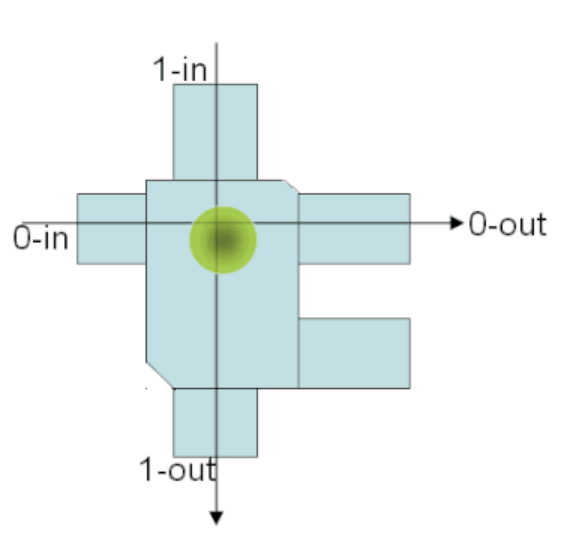
\includegraphics[width=0.7\textwidth]{2/single.png}};
\visible<1>{\fill[color=SpringGreen] (-.59,2.2) circle(0.25);}
\visible<2>{\fill[color=SpringGreen] (-.59,-2.1) circle(0.25);}
\visible<3>{\fill[color=SpringGreen] (-2.7,0.3) circle(0.25);}
\visible<4>{\fill[color=SpringGreen] (2.5,0.3) circle(0.25);}
\end{TIKZP}

}
\only<5->{
\MedSkip{}No energy is put in or taken out of the system.  The ball has its own energy, maintained throughout its motion through the box.}
    
\end{frame}
\begin{frame}{The billiard ball computer}{When two balls enter simultaneously}
\TwoUnequalColumns{0.6\textwidth}{0.4\textwidth}{%
Here, two balls enter, one from the top, and one from the left
\begin{itemize}
    \item<1-> A ball entering from the top and a ball entering from the left at the same time
    \only<2->{will \alert<2>{collide here}.}
    \item<3-> They bounce internally at the same time.
    \item<4-> One ball emerges from the ``AND-output'' chute and the other emerges from the ``1-out'' chute.
    
\end{itemize}
}{%
\Vskip{-3.2em}\Hskip{-0em}
\begin{TIKZP}
\node at (0,0)
    {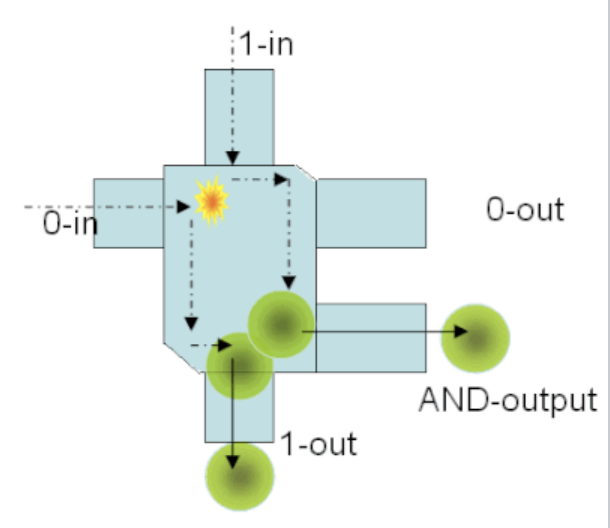
\includegraphics[width=0.7\textwidth]{2/double.png}};
\visible<1>{\fill[color=SpringGreen] (-.45,1.8) circle(0.25);}
\visible<2>{\fill[color=red] (-.6,0.4) circle(0.25);}
\visible<1>{\fill[color=SpringGreen] (-2.2,0.3) circle(0.25);}
\end{TIKZP}

}
\only<5->{
\SmallSkip{}Again, the energy of the box remains the same throughout.\Remark{It would take energy to \emph{stop} the ball from exiting the ``1-out'' chute.}}

    
\end{frame}

\section{Reversible gates}
\begin{frame}{Not and And}{From page 12 of \Kaye{}.}
\TwoColumns{%
\begin{itemize}
    \item<1-> The \emph{not} gate is reversible and is in fact its own inverse.
    \item<2-> Is \And{a}{b} reversible if we know $a$?  \only<3->{No.} \only<3>{If $a=0$, $b$ could be either $0$ or $1$.}
    \item<4-> We need a copy of both inputs to create a reversible \emph{and} gate.
\end{itemize}
 
}{%


\begin{center}
\only<1>{
\begin{GateBox}[scale=0.5]{2}{1}{1}
\BoxLabel{Not}
\Input{0}{$a$}
\Output{0}{\Overline{a}}
\end{GateBox}}

\only<2-3>{\begin{GateBox}{2.5}{1}{2}
\BoxLabel{Copy $a$/And}
\Input{0}{$a$}
\Input{1}{$b$}
\Output{0}{$a$}
\Output{1}{\And{a}{b}}
\end{GateBox}}


\only<4>{\begin{GateBox}{2.5}{1}{3}
\BoxLabel{Reversible?}
\Input{0}{$a$}
\Input{1}{$b$}
\Output{0}{$a$}
\Output{1}{$b$}
\Output{2}{\And{a}{b}}
\end{GateBox}}

\only<5>{\begin{GateBox}{2.5}{1.5}{3}
\BoxLabel{\mbox{\stackbox[c]{Reversible\\ And}}}
\Input{0}{$a$}
\Input{1}{$b$}
\Input{2}{\Zero{}}
\Output{0}{$a$}
\Output{1}{$b$}
\Output{2}{\And{a}{b}}
\end{GateBox}}
\end{center}
}
\MedSkip{}
   \only<4>{
    However, this box must generate energy to produce the third output.  To conserve energy, a reversible box must have the same number of inputs as outputs.}

\only<5>{This box enables reversal of the computation and it accepts an \href{https://en.wikipedia.org/wiki/Ancilla_bit}{ancilla} bit as a third input.}

\OnlyRemark{5}{The circuit elements involved in quantum computations must be \emph{reversible} and must contain the same number of inputs as outputs.}
\end{frame}

\begin{frame}{Common reversible gate used in quantum computing}{Uses the third input to greater advantage}
\TwoColumns{%
\begin{itemize}
    \item<1-> The signals $a$ and $b$ are copied to their respective outputs.
    \item<2-> The bottom output is computed as: 
    \only<2->{
    \Vskip{-2em}\begin{description}
        \item[$c=0$] The output is \And{a}{b}.
        \item[$c=1$] The output is \Nand{a}{b}.
    \end{description}}
    \item<3-> The gate is known in quantum computing as the \href{https://en.wikipedia.org/wiki/Toffoli_gate}{Tofolli Gate}.
\end{itemize}
}{%
\begin{center}
\begin{GateBox}{2.5}{1.5}{3}
\only<1-2>{\BoxLabel{\mbox{f(a,b)=\And{a}{b}}}}
\only<3-4>{\BoxLabel{Tofolli Gate}}
\only<5->{\BoxLabel{\mbox{\stackbox[c]{Tofolli Gate\\ CCNOT}}}}

\Input{0}{$a$}
\Input{1}{$b$}
\Input{2}{$c$}
\Output{0}{$a$}
\Output{1}{$b$}
\only<1-3>{\Output{2}{\Xor{c}{(\And{a}{b})}}}
\only<4->{\Output{2}{\Xor{(\And{a}{b})}{c}}}
\end{GateBox}
\end{center}
\only<4->{\MedSkip{}
An alternative view of this gate:
\begin{itemize}
    \item When $a$ and $b$ are both \True{}, the incoming signal $c$ is complemented on output.
    \item<5-> It is thus also called a controlled-controlled-Not gate, or CCNOT.
\end{itemize}
}
}
    
\end{frame}